% Todos los archivos .tex principales deberían comenzar con \documentclass
\documentclass[10pt]{article}

% Esto es para que el LaTeX sepa que el texto y tablas están en español
\usepackage[spanish, es-lcroman, es-tabla]{babel}

% Para que se reconozcan todos los caracteres
\usepackage[utf8]{inputenc}

% Para formato de citas con BibTeX
\usepackage{csquotes}

% Paquetes de la AMS para ampliar matemática
\usepackage{amsmath, amsthm, amsfonts, amssymb}

% Extensión de amsmath
\usepackage{mathtools}

% Para agregar una posibilidad de font matemático extra
\usepackage{mathrsfs}

% Paquete para escribir varias columnas
\usepackage{multicol}

% Paquete para uso de hipervínculos nativo
\usepackage{hyperref}

% Paquete para escribir codigo
\usepackage{listings}
% Opciones para permitir tildes en código
\lstset{
	basicstyle=\tiny\ttfamily,
    inputencoding=utf8,
    extendedchars=true,
    literate=%
	{á}{{\'a}}1
	{é}{{\'e}}1
	{í}{{\'i}}1
	{ó}{{\'o}}1
	{ú}{{\'u}}1
	{ü}{{\"u}}1
	{Á}{{\'A}}1
	{É}{{\'E}}1
	{Í}{{\'I}}1
	{Ó}{{\'O}}1
	{Ú}{{\'U}}1
    {Ü}{{\"U}}1
}

% Para incluir imagenes con más versatilidad
\usepackage{graphicx}

% Para generar subfiguras
\usepackage{subfig}

% Para poder controlar directamente lugar de figuras
\usepackage{float}

% Para agregar opciones al enumerate
\usepackage{enumitem}

% Para citar con facilidad
\usepackage[backend=biber, style=apa, sorting=nty]{biblatex}
\DeclareLanguageMapping{spanish}{spanish-apa}
\addbibresource{bibliografia.bib}  % Tu archivo de bibliografía

% Algunos ambientes matemáticos
\newtheorem{thm}{Teorema}[section]
\newtheorem{cor}[thm]{Corolario}
\newtheorem{lem}[thm]{Lema}
\newtheorem{prop}[thm]{Proposición}
\theoremstyle{definition}
\newtheorem{defn}[thm]{Definición}
\theoremstyle{remark}
\newtheorem{rem}[thm]{Observación}
\theoremstyle{definition}
\newtheorem{prob}{Problema}

% Abreviaciones para derivadas
\newcommand{\pd}[2]{\frac{\partial #1}{ \partial #2}}   % First partial derivative command
\newcommand{\td}[2]{\frac{\mathrm{d} #1}{ \mathrm{d} #2}}  % Derivada
\newcommand{\pdd}[2]{\frac{\partial^2 #1}{ \partial #2 ^2}}   % Second partial derivative command
\newcommand{\pddc}[3]{\frac{\partial^2 #1}{ \partial #2 \partial #3}}   % Cross partial derivative command

% Continuum mechanics & FEM symbols
\def\sca   #1{\mbox{\rm{#1}}{}}
\def\mat   #1{\mbox{\boldmath $\mathsf #1$}}
\renewcommand{\vec}[1]{\boldsymbol{#1}}
\newcommand{\ten}[1]{\boldsymbol{#1}}
\def\ltr   #1{\mbox{\sf{#1}}}
\def\bltr  #1{\mbox{\sffamily{\bfseries{{#1}}}}}

% Math operators and symbols
\DeclareMathOperator{\dive}{div}
\DeclareMathOperator{\tr}{tr}
\DeclareMathOperator{\symm}{symm}
\DeclareMathOperator{\sk}{skew}
\DeclareMathOperator{\grad}{grad}
\DeclareMathOperator{\Grad}{Grad}
\DeclareMathOperator{\curl}{curl}
\DeclareMathOperator{\Curl}{Curl}
\newcommand{\R}{\mathbb{R}}
\newcommand{\dx}{\, \mathrm{d}x}

% Para cambiar márgenes
\usepackage{geometry}
\geometry{left=2.5cm, right=2.5cm, top=2cm, bottom=3cm}

\begin{document}

\begin{titlepage}
	\begin{figure}
		\begin{minipage}{2cm}
			
\includegraphics[width=0.8\textwidth]{./figures/LogoUC-BN}
		\end{minipage}
		\begin{minipage}{14.5cm}
			\vspace{4mm}
			{\sc Pontificia Universidad Católica de Chile}\\
			Escuela de Ingeniería\\
			%Departamento de Ingeniería Estructural y Geotécnica\\
			%Instituto de Ingeniería Biológica y Médica\\
			{\bf ICE/IBM2020 Introducción a la Biomecánica}\\
			\vspace{0mm}
			\hrulefill
		\end{minipage}
	\end{figure}
	\phantom{""}\vspace{60mm}
	\begin{center}
		\Huge{\textbf{Tarea X}}\vspace{95mm}\\
		\raggedleft \Large{Nombre Apellido Apellido}\\
		XX de marzo de 2021\\
		Tiempo dedicado: XX
	\end{center}
\end{titlepage}

% Problema 1
\begin{prob} Consideramos la viga de la figura \ref{fig:viga}:

\begin{figure}[H] % Requiere package float
	\centering
	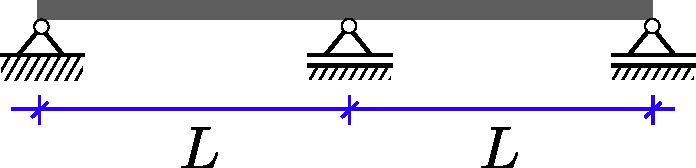
\includegraphics[width=0.3\textwidth]{./figures/Figura1}
	\caption{Esquema de viga.}
	\label{fig:viga}
\end{figure}

Para poder agregar la figura \ref{fig:viga} los comandos fueron:

\begin{verbatim}
	\begin{figure}[H] % Requiere package float
		\centering
		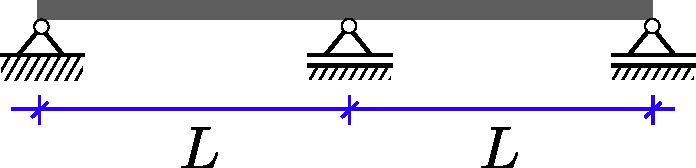
\includegraphics[width=0.3\textwidth]{./figures/Figura1}
		\caption{Problema 1}
		\label{fig:viga}
	\end{figure}
\end{verbatim}

Para escribir varios \textit{itemes} se utiliza
\begin{verbatim}
	\begin{enumerate}
		\item Ítem 1
		\item Ítem 2
	\end{enumerate}
\end{verbatim}

\begin{enumerate}
	\item Ítem 1
	\item Ítem 2
\end{enumerate}

\end{prob}

% Problema 2
\begin{prob} Aquí comienza el segundo problema.

\begin{figure}[H] % Requiere package float
	\centering
	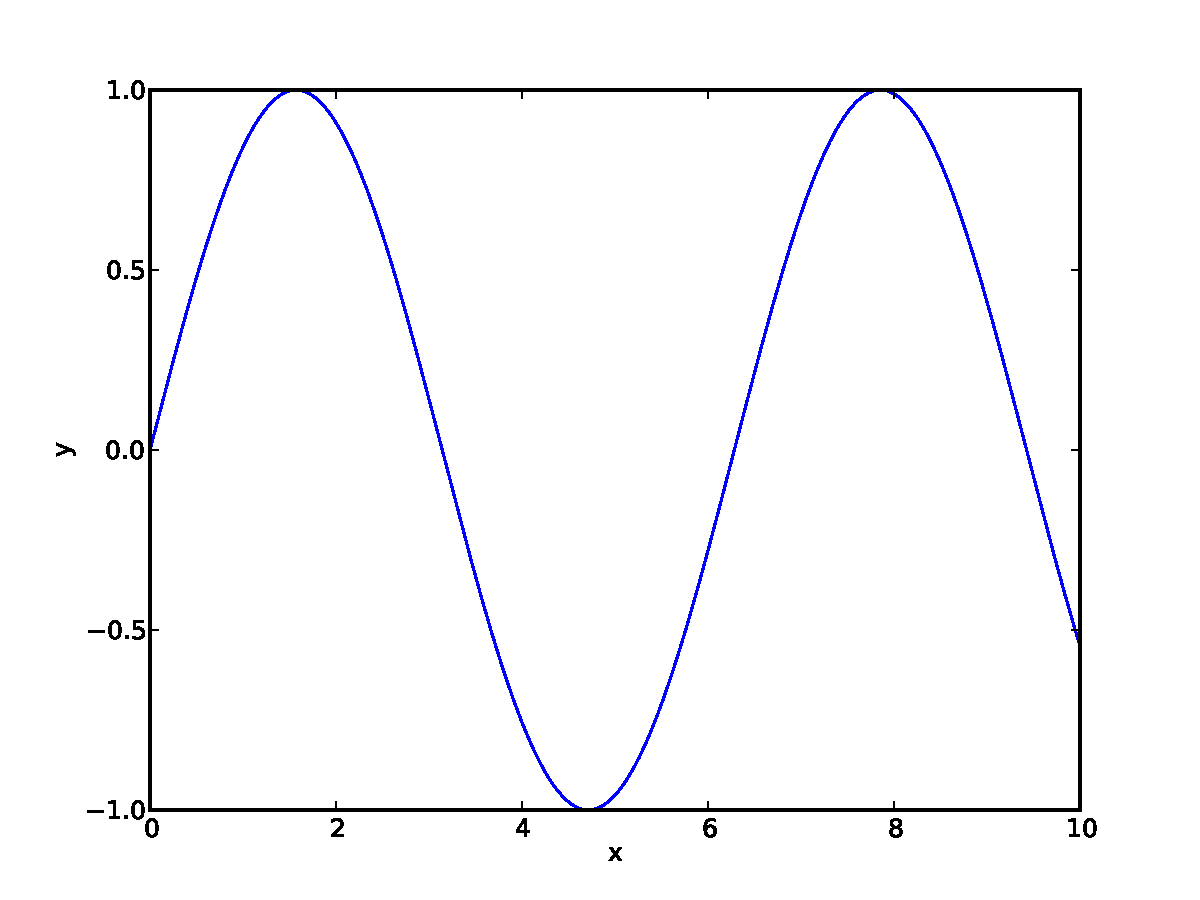
\includegraphics[width=0.8\textwidth]{./figures/sin}
	\caption{Función seno}
	\label{fig:seno}
	\end{figure}
\end{prob}

% Problema 3
\begin{prob} A continuación se muestra una tabla. Vea el código fuente disponible en el template para aprender a hacer tablas:

\begin{table}[H]
	\centering
	\begin{tabular}{||c|c|c|c||}  % Cada letra representa una columna. Las opciones son l, c y r (left, center, right)
		\hline  % hline crea una linea horizontal
		Tomate & Pera & Kiwi & Manzana \\
		\hline
		Naranja & Platano & Damasco & Durazno \\
		\hline
	\end{tabular}
	\caption{Distintas frutas y verdudas}
	\label{tab:frutas}
\end{table}
En la tabla \ref{tab:frutas} vemos los nombres de las frutas y verduras que se me ocurrieron al momento de hacer este template.

\end{prob}

% Problema 4
\begin{prob} Vamos a escribir una de las ecuaciones más bonitas del mundo. Esta es
\begin{equation}
	1 + e^{i\pi} = 0
	\label{eq:masbonita}
\end{equation}
conocida como la identidad de Euler.

La ecuación \eqref{eq:masbonita} es conocida como una de las ecuaciones más bellas del mundo porque tiene varios de los números más importantes de las matemáticas. Vamos a desarrollar un poco la expresión:
\begin{align}
	1+e^{i\pi} & = 1 + \cos \pi + i \sin \pi \\
	& = 1 + (-1) + i \cdot 0 \\
	& = 1 - 1 \\
	& = 0
\end{align}

En realidad no me gusta que todas las ecuaciones tengan número:
\begin{align*}  % El asterisco evita la enumeración
	1+e^{i\pi} & = 1 + \cos \pi + i \sin \pi \\
	& = 1 + (-1) + i \cdot 0 \\
	& = 1 - 1 \\
	& = 0
\end{align*}

Tampoco me gusta que ninguna tenga número, quiero que la última tenga número:
\begin{align}
	1+e^{i\pi} & = 1 + \cos \pi + i \sin \pi \nonumber \\
	& = 1 + (-1) + i \cdot 0 \nonumber \\
	& = 1 - 1 \nonumber \\
	& = 0
\end{align}

Una ecuación importante para un ingeniero:
\begin{equation}
	\rho \left(\pd{\vec{v}}{t} + \vec{v} \cdot \nabla \vec{v} \right) = - \nabla p + \nabla \cdot \ten{T} + \ten f
\label{eq:ns}
\end{equation}
conocida como la ecuación de Navier-Stokes.

Además de esto puedo definir matemática mientras escribo un párrafo. Sea $\vec{u} : \Omega \to \R^{3}$ un campo vectorial suave tal que
\begin{equation}
	\vec{u} \propto -\nabla p
\end{equation}
es decir, proporcional al gradiente negativo de $p$. Por último, puedo definir un conjunto de ecuaciones relacionadas, como
\begin{subequations}
	\label{eq:maxwell}
	\begin{align}
		\nabla \cdot \vec{E} & = \frac{\rho}{\varepsilon_{0}} \\
		\nabla \cdot \vec{B} & = 0 \\
		\nabla \times \vec{E} & = -\pd{\vec{B}}{t} \\
		\nabla \times \vec{B} & = \mu_{0} \left( \vec{J} + \varepsilon_{0} \pd{\vec{E}}{t} \right)
	\end{align}
\end{subequations}
y referirme a ellas como las ecuaciones \eqref{eq:maxwell}. Estas ecuaciones se conocen como las ecuaciones de Maxwell (\cite{wikipedia}) y verán que cité esa referencia, además de que la verán al final del texto.

Finalmente en el anexo pueden encontrar el código utilizado para generar la figura \ref{fig:seno}. Utilicen el paquete de \LaTeX listings para agregar el código de forma ordenada. Este template ya lo incluye, para que ustedes lo hagan en sus tareas.

Lean el template y verán como se llama a cada archivo.

\end{prob}

\newpage

\printbibliography

\newpage

\twocolumn
\begin{center}
	\textbf{Anexo: Códigos}
\end{center}

\lstinputlisting[language=Python]{./codes/sin.py}

\end{document}